%LaTeX Template 
%%	by	Xu Gao (gausyu@gmail.com)
%%LPPL: http://www.latex-project.org/lppl.txt
%------------------------
%The following is the Preamble
%------------------------
\documentclass[11pt]{article}
%This is the document class. 
%%	Most common: article, beamer, book, etc.
%%	11pt means the default font size is 11pt. One can also use 10pt, 11pt, or 12pt.
%%	See https://en.wikibooks.org/wiki/LaTeX/Document_Structure#Document_classes for explaination.
%------------------------
%Packages
%------------------------
\usepackage[a4paper,total={6in, 9in}]{geometry} 
%This aims to customize page layout
\usepackage[T1]{fontenc}
%Using T1 font
\usepackage[leqno]{mathtools}
%The main MATH package (for whom may wonder, mathtools load amsmath automatically, so no need \usepackage{amsmath})
\usepackage{amsthm}
%This defines the theorem enviroments
\usepackage{amssymb}
%Math symbols
\usepackage{bm}
%Bold math fonts, provide \bm{} command
\usepackage[scr=rsfs,cal=euler]{mathalpha}
%Math fonts 
%%The package provides means of loading maths alphabets (such as are normally addressed via macros \mathcal, \mathbb, \mathfrak and \mathscr)
%%How to use? "scr=" set what font \mathscr use, "cal=" set what font \mathcal use, "bb=" set what font \mathbb use, and "frak=" set what font \mathfrak use.
\usepackage{tikz}
\usetikzlibrary{automata}
\usetikzlibrary{arrows.meta}
\tikzset{>=latex}
%Drawing
\usepackage{graphicx}
%Support for graphics
\usepackage{hyperref}
\usepackage[nameinlink]{cleveref}
%Hyper links
\hypersetup{
	colorlinks=true,
	linkcolor=blue,
	urlcolor=magenta
}
%Color links
\usepackage{etoolbox}
%Programming
\usepackage[shortlabels]{enumitem}
%Enable enumerate modification
\usepackage{tcolorbox}
%provides an environment for coloured and framed text boxes with a heading line.
\tcbset{colback=white}
%------------------------
%Theorem-like Enviroments
%------------------------
\crefname{equation}{}{}
\theoremstyle{plain}
%This is the theorem style, plain means blod title and italic body
\newtheorem{theorem}{Theorem}
%This is how you define a theorem-like enviroment.
\newtheorem{lemma}[equation]{Lemma}
\newtheorem{proposition}[equation]{Proposition}
%The option [equation] means the lemmas are numbered following the same system of equation.
\newtheorem*{propstar}{Proposition}
%Star version defines unnumbered enviroments
\theoremstyle{definition}
%This is the theorem style, definition means blod title and normal body
\newtheorem*{defn}{Definition}
\newtheorem{example}[equation]{Example}
%The option [equation] means the examples are numbered following the same system of equation.
\newtheorem{problem}{Problem}
%This is the enviroment used as problems in HWs.
\theoremstyle{remark}
%This is the theorem style, remark means italic title and normal body
\newtheorem*{remark}{Remark}
\newtheorem*{hint}{Hint}
\newtheorem*{optional}{Optional}
%Remark enviroment
\numberwithin{equation}{problem}
%Let equations be numbered with in each problems.
\NewDocumentEnvironment{solution} {o} 
{\begin{proof}[\IfNoValueTF{#1}{\textbf{Solution}}{\textbf{Solution} (#1)}]}{\end{proof}}
%This defines the enviroment for you to write solutions.
%------------------------
\newlist{listinprob}{enumerate}{1}
\setlist[listinprob]{label=(\alph{listinprobi}),
                  ref=\theproblem.(\alph{listinprobi})}
\crefname{listinprobi}{problem}{problems}
\Crefname{listinprobi}{Problem}{Problems}
%This defines a new list type used in the enviroment problem.
%------------------------
%DocumentCommands
%------------------------
%Notations for number sets
\NewDocumentCommand \N {} { \mathbb{N} }%Natural numbers
\NewDocumentCommand \Z {} { \mathbb{Z} }%Integers
\NewDocumentCommand \Q {} { \mathbb{Q} }%Rational Numbers
\NewDocumentCommand \R {} { \mathbb{R} }%Real Numbers
\NewDocumentCommand \C {} { \mathbb{C} }%Complex Numbers
\NewDocumentCommand \F {} { \mathbb{F} }%Field
\NewDocumentCommand \scrO {} {	\mathscr{O}	}%Dedekind doamin
%Notations for maps
\DeclareMathOperator{\id}{id} % identity
\DeclareMathOperator{\pr}{pr} % projection
\DeclareMathOperator{\pt}{pt} % point
\DeclareMathOperator{\res}{res} % restriction
%PairedDelimiters
\DeclarePairedDelimiterX\abs[1]\lvert\rvert
  { \ifblank{#1}{\:\cdot\:}{#1} }
%abstract value function
\DeclarePairedDelimiterX\norm[1]\lVert\rVert
  { \ifblank{#1}{\:\cdot\:}{#1} }
%the norm function
\DeclarePairedDelimiterX\ceil[1]\lceil\rceil
  { \ifblank{#1}{\:\cdot\:}{#1} }
%ceil function
\DeclarePairedDelimiterX\floor[1]\lfloor\rfloor
  { \ifblank{#1}{\:\cdot\:}{#1} }
%floor function
\DeclarePairedDelimiterX\pairing[2]\langle\rangle
  { \ifblank{#1}{\:\cdot\:}{#1}, \ifblank{#2}{\:\cdot\:}{#2} }
\DeclarePairedDelimiterX\inner[2]\lparen\rparen
  { \ifblank{#1}{\:\cdot\:}{#1}, \ifblank{#2}{\:\cdot\:}{#2} }
%Inner product
\providecommand\given{}
\newcommand\SetSymbol[1][]
  { \nonscript\:#1\vert\allowbreak\nonscript\:\mathopen{} }
\DeclarePairedDelimiterX\Set[1]\{\}
  { \renewcommand\given{\SetSymbol[\delimsize]}#1 }
%a set
%
%Miscellaneous
\NewDocumentCommand \vect { m } { \mathbf{#1} }
%Vector
\RenewDocumentCommand \le {} { \leqslant }
\RenewDocumentCommand \ge {} { \geqslant }
%Change the inequality symbols
\NewDocumentCommand \tforall {} {\quad\text{for all}\quad}
%------------------------
% Additional math symbols, used for the Math 110 course
\DeclareMathOperator*\GCD{GCD}
\DeclareMathOperator*\LCM{LCM}
\usepackage{derivative}% Support typing calculus notations.
%------------------------
\allowdisplaybreaks
%Allow a long equation to display in more than one page.

%The following change the default layout of title
\makeatletter
\def\@maketitle{%
	\newpage
	\null
	\vskip 2em%
	\begin{center}%
		\let \footnote \thanks
		\sffamily 
		{\LARGE \@title \par}%
		\vskip 1.5em%
		{\large \@subtitle \par}%
		\vskip 1.5em%
		{\large Student name: \@author \par}%
		\ifdefempty{\@acknowledge}{}%
		{\large With help of: \@acknowledge \par}%
		\vskip 1em%
		{\large \@date}%
	\end{center}%
	\par
	\vskip 1.5em%
}	
\global\let\@subtitle\@empty
\DeclareRobustCommand*{\subtitle}[1]{\gdef\@subtitle{#1}}
\global\let\@acknowledge\@empty
\DeclareRobustCommand*{\acknowledge}[1]{\gdef\@acknowledge{#1}}
\makeatother
%Leave this change alone if you don't know what it means

%%%
%%%	START WORKS
%%%
%------------------------
%Information of the file
%------------------------
\title{Homework 5 (due Nov. 8)}
%The title of the file
\author{[Your Full Name Here]}
%Input your full name here.
% \acknowledge{[Your collaborators]}
%Input your collaborators, if none, comment it.
\subtitle{MATH 110~|~Introduction to Number Theory~|~Fall 2022}
%The subtitle
\date{\today} 
%The date, if commented, the value will be \today
 
%------------------------
%Document starts here
%------------------------
\begin{document}
\maketitle

\begin{problem}
	\begin{listinprob}
		\item	(5 pts) What are \textbf{all} the possible natural representatives of $n^2\pmod 8$, where $n$ is an integer.
%----------------------------------------
\begin{solution} %Do not delete
WRITE YOUR SOLUTION HERE
\end{solution}\clearpage %Do not delete
%----------------------------------------

		\item (5 pts) Determine whether the following equation is solvable in $\Q$ or not? If it is, \textbf{find} such a solution $(x,y,z)\in\Q^3$, if not, \textbf{prove it}.
		\[
			x^2+y^2+z^2=2023
		\] 
		\begin{hint}
			First translate it into a Diophantine equation asking solutions in $\Z$. Then consider the congruence modulo $8$. 
		\end{hint}
	\end{listinprob}	
\end{problem}
%----------------------------------------
\begin{solution} %Do not delete
WRITE YOUR SOLUTION HERE
\end{solution}\clearpage %Do not delete
%----------------------------------------

\begin{problem}
	Let $p$ be any prime number and let $a$ and $b$ be any two integers.
	\begin{listinprob}
	\item (5 pts) Prove that if $a \equiv b \pmod{p}$, then $a^p \equiv b^p \pmod{p^2}$.
%----------------------------------------
\begin{solution} %Do not delete
WRITE YOUR SOLUTION HERE
\end{solution}\clearpage %Do not delete
%----------------------------------------

	\item (5 pts) Prove that if $a \equiv b \pmod{p}$, then $a^{p^2} \equiv b^{p^2} \pmod{p^3}$.
%----------------------------------------
\begin{solution} %Do not delete
WRITE YOUR SOLUTION HERE
\end{solution}\clearpage %Do not delete
%----------------------------------------

	\item (Optional, up to 5 extra pts) Can you generalise?
	\end{listinprob}
\end{problem}
%----------------------------------------
\begin{solution} %Do not delete
WRITE YOUR SOLUTION HERE
\end{solution}\clearpage %Do not delete
%----------------------------------------

\begin{problem}[10 pts]
	Solve the congruences $5x \equiv 11\pmod{37}$ and $11y \equiv 5\pmod{37}$. 
\end{problem}

\begin{problem}
	Consider the following modular dynamical system, which is neither additive nor multiplicative.
	\begin{listinprob}
	\item (5 pts) Let $X = \Z/13$ and let $f : X \to X$ be given by
	\[x \mapsto f(x) \coloneqq x^2 + 3 \pmod{13}.\]
	Draw the complete diagram for the dynamics of $f$.
%----------------------------------------
\begin{solution} %Do not delete
	The complete diagram for the dynamics of $f$ is the following:
	\begin{center}
		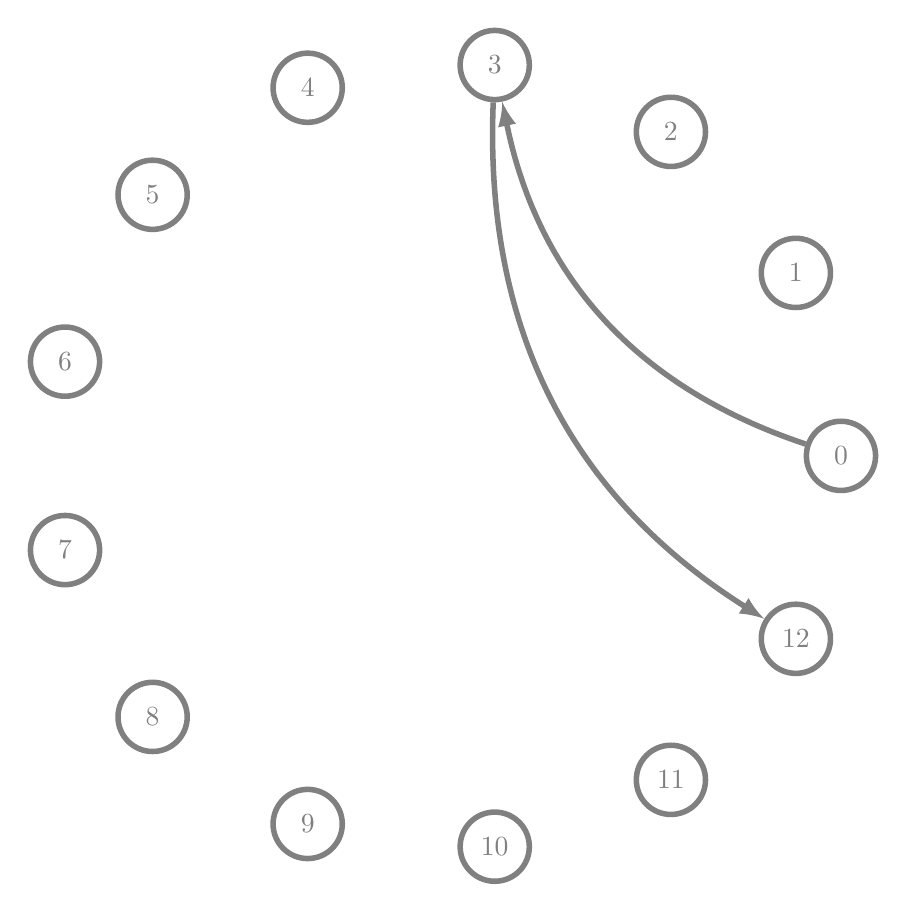
\begin{tikzpicture}[nodes=state,every path/.append style={->,line width=2pt,gray}]
			\def \number {13}
			\def \radius {5cm}
			\def \degree {360/\number}
			\foreach \i [count=\j from 0] in {1,...,\number}
				{
					\node at ({\degree * \j}:\radius) (\j) {$\j$};
				}
%-----Draw the arrows here-----
			\path (0) edge[bend left] (3);%An arrow from 0 to 3
			\path (3) edge[bend right] (12);%An arrow from 3 to 12
			%COMPLETE the diagram by filling the rest 11 arrows.
		\end{tikzpicture}
	\end{center}
\end{solution}\clearpage %Do not delete
%----------------------------------------

	\item (5 pts) Let $A_0 = 0$ and let $A_{n+1} = f(A_n) \pmod{13}$ for all integers $n \geq 0$. What is $A_{2022} \pmod{13}$?
	\end{listinprob}
\end{problem}
%----------------------------------------
\begin{solution} %Do not delete
WRITE YOUR SOLUTION HERE
\end{solution}\clearpage %Do not delete
%----------------------------------------

\begin{problem}[10 pts]
	Compute the length of the cycles in the dynamics of \fbox{$\times a \pmod{8}$} for every $a \in \Phi(8)$. Compare the length with $\varphi(8)$ (in the sense of divisibility or equality).
\end{problem}
%----------------------------------------
\begin{solution} %Do not delete
WRITE YOUR SOLUTION HERE
\end{solution}\clearpage %Do not delete
%----------------------------------------

\begin{thebibliography}{9}  %Do not delete
	%List your references here
	\bibitem[TEXT]{texbook}
	\emph{An Illustrated Theory of Numbers}, Martin H. Weissman.
	
	\bibitem[label]{citekey}
	[Book(s): \emph{Title}, Author ] or [Online: \href{http://example.com/}{Link}]
\end{thebibliography}  %Do not delete
%------------------------
\end{document}
